\documentclass{article}

%% Font related
\renewcommand{\familydefault}{\sfdefault}
\usepackage[T1]{fontenc}

%% Document related
\usepackage[utf8]{inputenc}
\usepackage[english]{babel}
\usepackage[margin=0.5in]{geometry}
\usepackage{flushend}

%% Table related
\usepackage{tabularx}

%% Maths related 
\usepackage{mathtools}

%% Figure related packages
\usepackage{graphicx}
\usepackage{float}

\usepackage{multicol}
\setlength{\columnsep}{1cm}

%% Document Sections related
\usepackage{titlesec}
\usepackage{tikz}
\usetikzlibrary{shapes.misc}
\newcommand\titlebar{%
\tikz[baseline,trim left=3.1cm,trim right=3cm] {
    \fill [cyan!25] (2.5cm,-1ex) rectangle (\textwidth-\textwidth/3, 2.5ex);
    \node [
        fill=cyan!60!white,
        anchor= base east,
        rounded rectangle,
        minimum height=3.5ex] at (3cm,0) {
        \textbf{\thesection.}
    };
}%
}
\titleformat{\section}{\large}{\titlebar}{0.1cm}{}
\renewcommand*{\thesection}{\arabic{section}}


\title{
  \textbf{Hadoop}\\
  \Large{reference card}
}
\author{Paulo Monteiro}
\begin{document}
\begin{multicols}{2}
\maketitle



%%%%%%%%%%%%%%%%%%%%%%%%%%%%%%
% Introduction
%%%%%%%%%%%%%%%%%%%%%%%%%%%%%%
\section{Introduction}
Hadoop is an open source distributed framework built to execute applications that process big data. \\
Some of its characteristics are:
\begin{itemize}
\item \textbf{Accessible:} by running on a cloud of computing services such as the Amazon Elastic Compute Cloud (EC2)
\item \textbf{Robust:} the redundancy of data allows Hadoop to recover should a single node fail
\item \textbf{Scalable:} scales out to handle larger data
\item \textbf{Simple:} by easily allowing parallel code
\item \textbf{Offline Processing:} it is designed for offline processing and analysis of large-scale data 
\item \textbf{key/value pairs:} uses key/value pairs as its basic data unit
\item \textbf{MapReduce model:} Under the MapReduce model, the data processing primitives are called mappers and reducers
\end{itemize}

\subsection{Hadoop as a distributed system}

With Hadoop, a data set is divided into smaller (typically 64 MB) blocks that are spread among many machines in the cluster via the Hadoop Distributed File System (HDFS). 
\begin{itemize}
\item Hadoop focuses on moving code (MapReduce programs to be executed) to data instead of vice versa 
\item By using distributed storage and transferring code instead of data, Hadoop avoids the costly transmission step when working with large data sets.
\item Hadoop employs a master/slave architecture for both distributed storage and distributed computation 
\item The distributed storage system is called the Hadoop File System (HDFS). 
\end{itemize}

\subsection{How it started}
\begin{itemize}
\item Around 2004, Google published two papers describing the Google File System (GFS) and the MapReduce framework
\item Hadoop started out as a subproject of Nutch, which in turn was a subproject of Apache Lucene
\item The Hadoop project was lead by Doug Cutting who saw an opportunity to develop an open source version of Google's MapReduce system
\end{itemize}



%%%%%%%%%%%%%%%%%%%%%%%%%%%%%%
% Understanding MapReduce
%%%%%%%%%%%%%%%%%%%%%%%%%%%%%%
\section{Understanding MapReduce}
MapReduce programs are executed in two main phases:
\begin{itemize}
\item \textbf{Mapping:} 
\subitem - The processing function is called \textbf{mapper}
\subitem - Takes the input data and feeds each data element to the mapper (\emph{filters} and \emph{transforms} the input)
\item \textbf{Reducing:} 
\subitem - The processing function is called \textbf{reducer}
\subitem - The reducer processes all the outputs from the mapper and arrives at a final result (\emph{aggregates})
\end{itemize}

MapReduce uses lists and (key/value) pairs as its main data primitives.\\
In the MapReduce framework you write applications \underline{by specifying the mapper and reducer}.\\\\
Here is the complete flow:
\begin{enumerate}
\item The input to the application must be structured as a list of (key/value) pairs, list(<k1, v1>)
\item The list of (key/value) pairs is broken up and each individual (key/value) pair, <k1, v1>, is processed by calling the map function of the mapper.
\item The mapper transforms each <k1,v1> pair into a list of <k2, v2> pairs.
\item The output of all the mappers are (conceptually) aggregated into one giant list of <k2, v2> pairs. All pairs sharing the same k2 are grouped together into a new (key/value) pair, <k2, list(v2)> .
\end{enumerate}

%%%%%%%%%%%%%%%%%%%%%%%%%%%%%%
% Hadoop Requirements
%%%%%%%%%%%%%%%%%%%%%%%%%%%%%%
\section{Hadoop Requirements}
\begin{itemize}
\item Linux is the official development and production platform/OS for Hadoop
\item Running Hadoop requires Java (>= version 1.6)
\item Running Hadoop on a single machine is mainly useful for development work
\item The command to run an Hadoop program is \emph{/bin/hadoop jar <jar>}
\end{itemize}

\newpage
\pagebreak

%%%%%%%%%%%%%%%%%%%%%%%%%%%%%%
% The building blocks
%%%%%%%%%%%%%%%%%%%%%%%%%%%%%%
\section{The building blocks}

"Running Hadoop” means running a set of daemons which include:
\begin{itemize}
\item NameNode
\item DataNode
\item Secondary NameNode
\item JobTracker
\item TaskTracker
\end{itemize}

\subsection {NameNode}
\begin{itemize}
\item Arguably the most vital of the Hadoop daemons
\item The NameNode is the master of HDFS that directs the slave DataNode daemons to perform the low-level I/O tasks
\item The function of the NameNode is memory and I/O intensive.
\end{itemize}

\subsection {DataNode}
\begin{itemize}
\item Each slave machine in the cluster will host a \textbf{DataNode daemon}
\item Responsible for reading and writing HDFS blocks to actual files on the local filesystem
\item \textbf{DataNodes} are constantly reporting to the \textbf{NameNode}
\end{itemize}

\subsection {Secondary NameNode}
\begin{itemize}
\item \textbf{The Secondary NameNode (SNN)} is an assistant daemon for monitoring the state of the cluster HDFS. 
\item Each cluster has one SNN and it typically resides on its own machine as well.
\end{itemize}

\subsection {JobTracker}
\begin{itemize}
\item The \textbf{JobTracker} daemon is the liaison between our application and Hadoop. \\Once
you submit your code to your cluster, it oversees the overall execution of the MapReduce job
\item There is only one JobTracker daemon per Hadoop cluster
\end{itemize}

\subsection {TaskTracker}
\begin{itemize}
\item The \textbf{TaskTrackers} manages the execution of individual tasks on each slave node
\item Each TaskTracker is responsible for executing the individual tasks that the JobTracker assigns
\item Each TaskTracker can spawn multiple JVMs to handle many map or reduce tasks in parallel
\item If the JobTracker fails to receive a heartbeat from a TaskTracker within a specified amount of time, it will assume the TaskTracker has crashed and will resubmit the corresponding tasks to other nodes in the cluster\\
\end{itemize}

We depict the topology of one typical Hadoop cluster:
\begin{figure}[H]
\centering
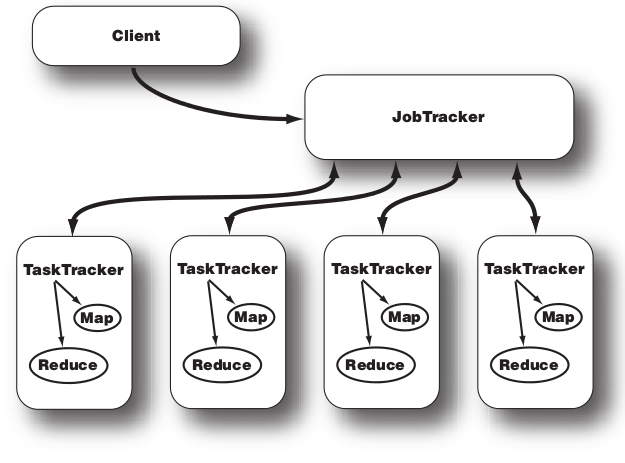
\includegraphics[width=7.5cm]{assets/jobTrackers_taskTrakers_diagram.png}
\caption{JobTracker and TaskTracker interaction}
\label{fig:awesome_image}
\end{figure}

\begin{figure}[H]
\centering
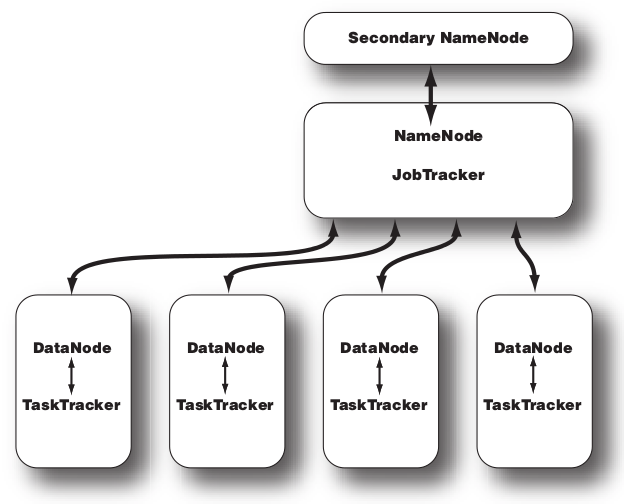
\includegraphics[width=7.5cm]{assets/cluster_topology.png}
\caption{Topology of a typical Hadoop cluster}
\label{fig:awesome_image}
\end{figure}


%%%%%%%%%%%%%%%%%%%%%%%%%%%%%%
% Running Hadoop
%%%%%%%%%%%%%%%%%%%%%%%%%%%%%%
\section{Running Hadoop}
\subsection {Local (Standalone) mode}
The default mode for Hadoop\\
Doesn’t use HDFS and will not launch any of the Hadoop daemons\\
\subsection {Pseudo-distributed mode}
This mode complements the standalone mode for debugging your code, allowing you to examine memory usage, HDFS input/output issues, and other daemon interactions.
\subsection {Fully distributed mode}
A full cluster setup.
\newpage
\pagebreak


%%%%%%%%%%%%%%%%%%%%%%%%%%%%%%
% Components of Hadoop
%%%%%%%%%%%%%%%%%%%%%%%%%%%%%%
\section{Components of Hadoop}
\subsection {Working with files in HDFS}
\begin{itemize}
\item HDFS is a filesystem designed for large-scale distributed data processing under frameworks such as MapReduce
\item HDFS abstracts details away and gives you the illusion that you’re dealing with only a single file
\item Hadoop provides a set of command line utilities that work similarly to the Linux file commands
\end{itemize}
\subsubsection {Basic file commands}
Hadoop fi le commands take the form of\\\\
\emph{\textbf{hadoop fs -cmd <args>}}\\
\begin{itemize}
\item The command \emph{\textbf{cmd}} is usually named after the corresponding Unix equivalent
\item Hadoop file commands can interact with both the HDFS filesystem and the local filesystem
\item HDFS defaults to a current working directory of \emph{/user/\$USER}, where \emph{\$USER} is your login user name.
\end{itemize}

\subsubsection {Operations with Files and Directories}
\begin{itemize}
\item hadoop fs –mkdir /user/chuck
\item hadoop fs -ls /
\item hadoop fs -put example.txt . (\emph{copy files from the local system into HDFS})
\item hadoop fs -get example.txt . (\emph{copies files from HDFS to the local filesystem})
\item hadoop fs -cat example.txt | head (\emph{Hadoop in conjuction with Unix pipes})
\item hadoop fs –rm example.txt
\item hadoop fs –help ls (\emph{Looking up help})
\end{itemize}


\subsection{Anatomy of a \emph{MapReduce} Program}
MapReduce program processes data by manipulating (key/value) pairs in the general form:\\\\
$map: (K1,V1) -> list(K2,V2)$\\
$reduce: (K2,list(V2)) -> list(K3,V3)$\\
\begin{figure}[H]
\centering
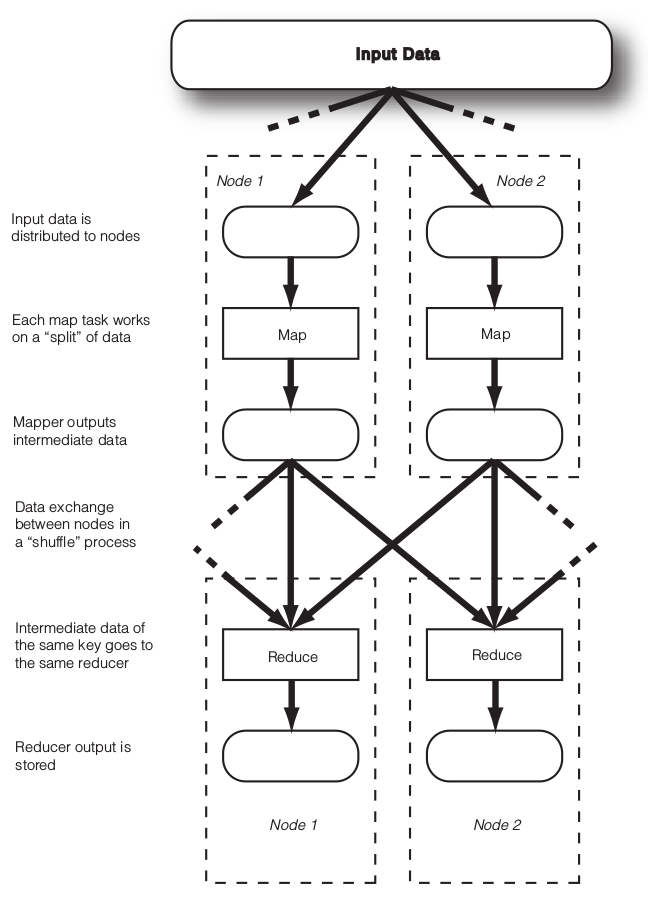
\includegraphics[width=9cm]{assets/anatomy.png}
\caption{The general MapReduce data flow.}
\label{fig:awesome_image}
\end{figure}

\subsection {Hadoop data types}
\begin{itemize}
\item \underline{Classes that implement the \emph{\textbf{Writable}} interface} can be values
\item \underline{Classes that implement the \textbf{WritableComparable<T>}} interface can be either keys or values
\item Hadoop comes with a number of predefined classes that implement \textbf{WritableComparable}:
\begin{figure}[H]
\centering
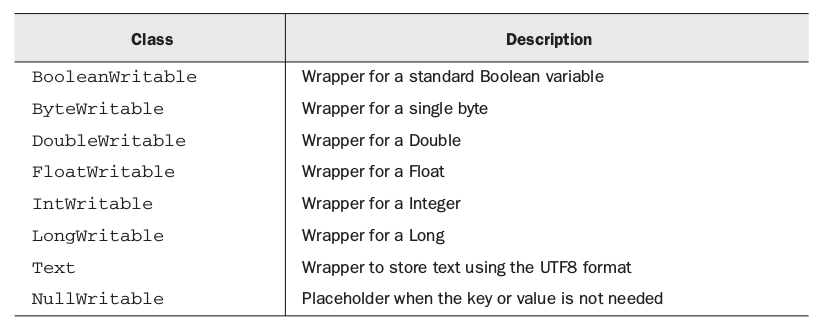
\includegraphics[width=9cm]{assets/data_types.png}
\caption{List of frequently used types for the key/value pairs.}
\label{fig:awesome_image}
\end{figure}
\end{itemize}


\subsection {Mapper}
\begin{itemize}
\item To serve as the mapper, a class must implement the \emph{\textbf{Mapper} interface} and inherit the \textbf{MapReduceBase} class.
\end{itemize}
\textbf{void configure(JobConf job)} 
\begin{itemize}
\item In this function you can extract the parameters set either by the configuration XML files or in the main class of your application.
\item Call this function before any data processing begins.
\end{itemize}
\textbf{void close()}
\begin{itemize}
\item As the last action before the map task terminates, this function should wrap up any loose ends
\end{itemize}
\textbf{void map(K1 key, V1 value,
                  OutputCollector<K2,V2> output,
                  Reporter reporter)}
\begin{itemize}
\item Generates a list of (K2, V2) pairs for a given (K1, V1) input pair.
\item The OutputCollector receives the output of the mapping process.
\item The Reporter provides the option to record extra information about the mapper as the task progresses.
\end{itemize}

\begin{figure}[H]
\centering
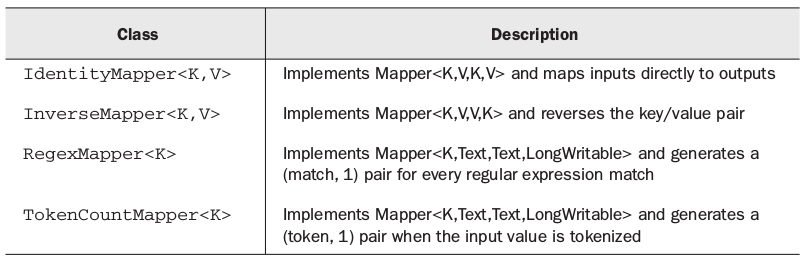
\includegraphics[width=9cm]{assets/mapper_functions.png}
\caption{Predefined Mapper implementations by Hadoop}
\label{fig:awesome_image}
\end{figure}


\subsection {Reducer}
\begin{itemize}
\item A reducer must extend the \textbf{MapReduce} base class
\end{itemize}
\textbf{void reduce(K2 key, Iterator<V2> values, OutputCollector<K3,V3> output, Reporter reporter ) }
\begin{itemize}
\item generates list of (K3, V3) pairs by iterating over the values associated with a given key. 
\item The OutputCollector receives the output of the reduce process and writes it to an output file. 
\item The Reporter provides the option to record extra information about the reducer as the task progresses.
\end{itemize}
\begin{figure}[H]
\centering
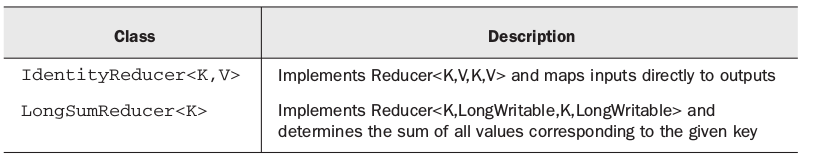
\includegraphics[width=9cm]{assets/reducer_impl.png}
\caption{Predefined Reducer implementations by Hadoop}
\label{fig:awesome_image}
\end{figure}

\subsection {Partitioner— redirecting output from Mapper}
\begin{itemize}
\item With multiple reducers, we need some way to determine the appropriate one to send a (key/value) pair outputted by a mapper
\item The default behavior is to \underline{hash the key to determine the} \underline{reducer}
\item Hadoop enforces this strategy by use of the \textbf{HashPartitioner class}
\item A custom partitioner only needs to implement two methods: 
\subitem \textbf{configure()} -  Uses the Hadoop job configuration to configure the partitioner 
\subitem \textbf{getPartition()} - Returns an integer between 0 and the number of reduce tasks indexing to which reducer the (key/value) pair will be sent.
\item Between the map and reduce stages, a MapReduce application must take the output from the mapper tasks and distribute the results among the reducer tasks. This process is typically called \textbf{shuffling}
\end{itemize}

\begin{figure}[H]
\centering
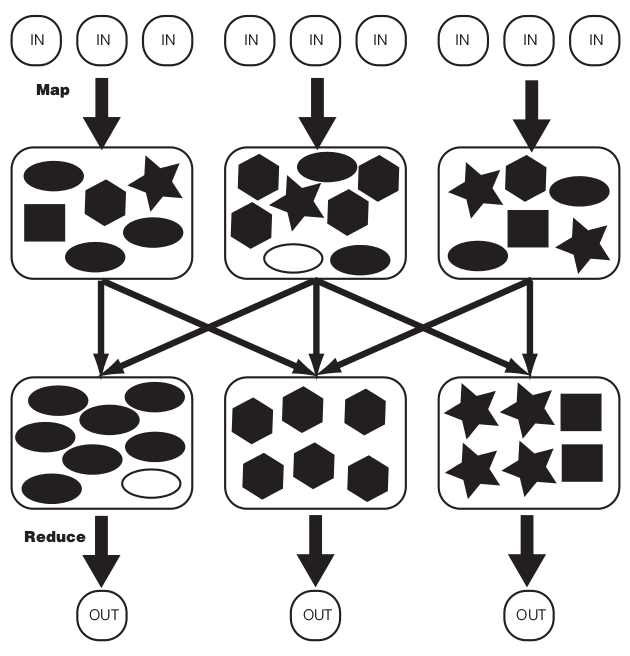
\includegraphics[width=9cm]{assets/partitioning.png}
\caption{The MapReduce data flow, with an emphasis on partitioning and shuffling. Each icon is a key/value pair. The shapes represents keys, whereas the inner patterns represent values. After shuffling, all icons of the same shape (key) are in the same reducer. Different keys can go to the same reducer, as seen in the rightmost reducer. The partitioner decides which key goes where}
\label{fig:awesome_image}
\end{figure}

\subsection {Combiner—local reduce}
In some situations, we may wish to perform a \emph{“local reduce”} before we distribute the mapper results.

\subsection {Reading and writing}
\begin{itemize}
\item One of the fundamental principles of MapReduce’s processing power is the splitting of the input data into chunks
\item In Hadoop terminology these chunks are called "\textbf{\emph{input splits}}"
\item In practice, a split usually ends up being the size of a block, which defaults to 64 MB in HDFS
\item Note that input splits are a logical division of your records whereas HDFS blocks are a physical division of the input data.
\end{itemize}

\subsection{InputFormat}
\begin{itemize}
\item The way an input file is split up and read by Hadoop is defined by one of the implementations of the \emph{\textbf{InputFormat} interface}. 
\item \textbf{TextInputFormat} is the default \textbf{InputFormat} implementation
\end{itemize}
\begin{figure}[H]
\centering
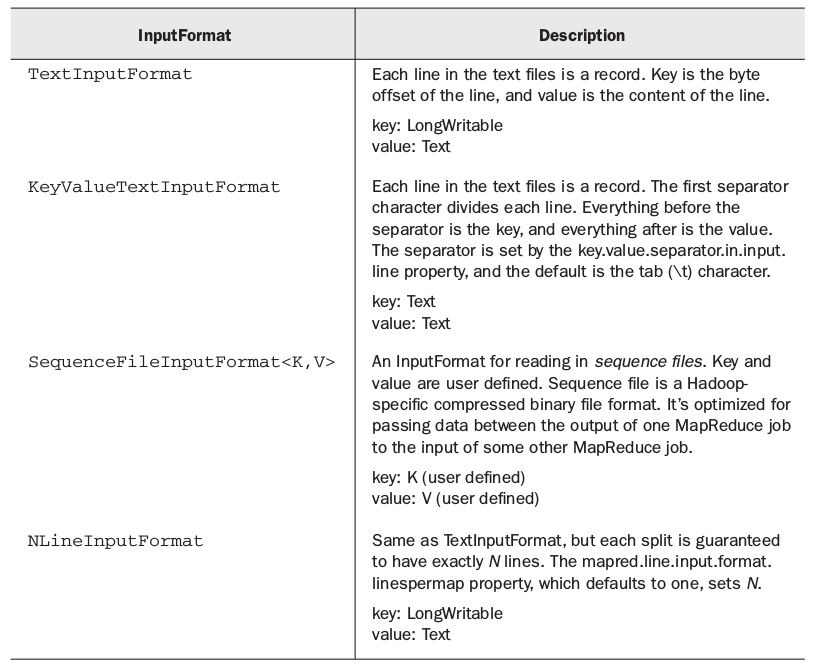
\includegraphics[width=9.5cm]{assets/popular_input.png}
\caption{Popular InputFormat classes}
\label{fig:awesome_image}
\end{figure}

\subsection{OutFormat}
\begin{itemize}
\item MapReduce outputs data into files using the \emph{\textbf{OutputFormat} class}. 
\item The output has no splits, as each reducer writes its output only to its own file
\item The output files reside in a common directory and are typically named \emph{part-nnnnn}, where nnnnn is the partition ID of the reducer
\item \textbf{RecordWriter} objects format the output and \textbf{RecordReader} parses the format of the input.
\item Almost all implementations of OutputFormat inherit from the \textbf{FileOutputFormat} abstract class
\item \textbf{SequenceFileInputFormat} it’s useful for writing intermediate data results when chaining MapReduce jobs.
\end{itemize}
\begin{figure}[H]
\centering
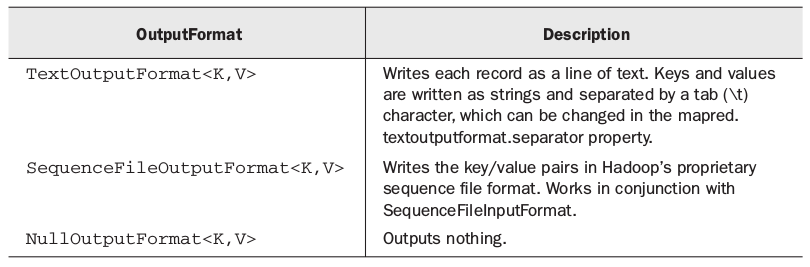
\includegraphics[width=9.5cm]{assets/popular_output.png}
\caption{Main OutputFormat classes. TextOutputFormat is the default}
\label{fig:awesome_image}
\end{figure}


\newpage
\pagebreak


\end{multicols}
\end{document}
